\documentclass[12pt]{article}
 
\usepackage[utf8]{inputenc}
\usepackage[T1]{fontenc}
\usepackage[francais]{babel}
\usepackage{enumerate}
\usepackage{listings}
\usepackage{xcolor}
\usepackage{graphicx}
\usepackage{amssymb}
\usepackage{amsmath}
\usepackage{geometry}
\usepackage{float}
\usepackage{tikz}

\geometry {
	left = 2.5cm,
	right = 2.5cm,
	bottom = 2.5cm ,
	top = 2.5cm ,
}

\lstdefinestyle{customjava}{
 belowcaptionskip=1\baselineskip,
 breaklines=true,
 frame=single,
 %linewidth=7.5cm,
 framexleftmargin=5mm,
 %frameround=tttt,
 %framexrightmargin=5mm,
 xleftmargin=\parindent,
 language=C++,
 showstringspaces=false,
 basicstyle=\footnotesize\ttfamily,
 keywordstyle=\color{green!40!black},
 ndkeywordstyle=\color{orange},
 commentstyle=\color{purple!40!black},
 identifierstyle=\color{blue},
 stringstyle=\color{red},
 %numbers=left,
 %numbersep=7pt,
}
%06/06/14
\frenchbsetup{StandardLists=true}
\title {Rapport : Format de Fichiers}
\author {Benjamin \emph{VANTHONG}}

\lstset{style=customjava, emph={int,double,void, Double}, emphstyle=\color{red}, emph={[2]wavJava, Spectrum}, emphstyle=[2]\color{orange}}
\begin{document}
\maketitle 
\section {Exportation d'un maillage au format HDF5}
En lisant la documentation XDMF, je me suis rendu compte que je devais changer la manière de stocker les données. En effet les coordonnées d'un  point du maillage doivent être stockées en ligne, et de même pour la liste des identifiants des noeuds qui décrivent un élément.\newline

Voici la méthode qui écrit les points :
\begin{lstlisting}
template <typename MeshType>
void Exporterhdf5<MeshType>::writePoints () 
{
    auto pt_it = M_meshOut->beginPointWithProcessId () ;
    auto const pt_en = M_meshOut->endPointWithProcessId () ;
    M_maxNumPoints= std::distance (pt_it, pt_en) ;

    hsize_t currentSpaceDims [2] ;
    hsize_t currentCount [2] ;

    currentSpaceDims[0] = 1;
    currentSpaceDims[1] = M_maxNumPoints ;

    currentCount[0] = M_maxNumPoints ;
    currentCount[1] = 3 ;

    M_HDF5.createTable ("point_coords", H5T_IEEE_F64BE, currentCount) ;
    M_HDF5.createTable ("point_ids", H5T_STD_U32BE, currentSpaceDims) ;

    M_uintBuffer.resize (currentSpaceDims[0]*currentSpaceDims[1], 0) ;
    M_realBuffer.resize (currentCount[0]*currentCount[1], 0) ;

    for (size_type i = 0 ; i < M_maxNumPoints ; i++ , pt_it++) 
    {
        M_uintBuffer[i] = pt_it->id () ;

        M_realBuffer[3*i] = pt_it->node()[0] ;
        if (mesh_type::nRealDim >= 2)
            M_realBuffer[3*i + 1] = pt_it->node()[1] ;
        if (mesh_type::nRealDim >= 3)
            M_realBuffer[3*i + 2] = pt_it->node()[2] ;
    }

    bubbleSort (&M_uintBuffer[0], &M_realBuffer[0], M_maxNumPoints) ;

    hsize_t currentOffset[2] = {0, 0} ;

    M_HDF5.write ("point_coords", H5T_NATIVE_DOUBLE, currentCount, currentOffset, &M_realBuffer[0]) ;
    M_HDF5.write ("point_ids", H5T_NATIVE_LLONG, currentSpaceDims, currentOffset , &M_uintBuffer[0]) ;


    M_HDF5.closeTable("point_coords") ;
    M_HDF5.closeTable("point_ids") ;
}
\end{lstlisting}
Dans le format \emph{xdmf} les identifiants des points en entrées doivent être ordonnés et comme ce n'est pas toujours le cas des maillages sous feel++ c'est pourquoi avant de stocker les données, on éffectue un tri à bulle. Cette méthode trie le tableau des identifiants et des coordonnées simultanément. \newline
Voici l'implémentation de ce tri :
\begin{lstlisting}
template <typename MeshType>
void Exporterhdf5<MeshType>::bubbleSort (size_type * ids, value_type * coords, size_type n) 
{
    size_type int_tmp ;
    value_type float_tmp ;
    bool swapped = false ;
    do 
    {
        swapped = false ;
        for (size_type j = 0 ; j < n-1 ; j ++) 
        {
            if (ids[j] > ids[j+1]) 
            {
                int_tmp = ids[j] ;
                ids[j] = ids[j+1] ;
                ids[j+1] = int_tmp ;

                float_tmp = coords[3*j] ;
                coords[3*j] = coords [3*(j+1)] ;
                coords[3*(j+1)] = float_tmp ;

                float_tmp = coords[3*j+1] ;
                coords[3*j+1] = coords [3*(j+1)+1] ;
                coords[3*(j+1)+1] = float_tmp ;

                float_tmp = coords[3*j+2] ;
                coords[3*j+2] = coords [3*(j+1)+2] ;
                coords[3*(j+1)+2] = float_tmp ;

                swapped = true ;
            }
        }
        n = n -1 ;
    }
    while (swapped) ;
}
\end{lstlisting}
Sous \textbf{Feel++} les identifiants des points commencent par un or en xdmf, ils doivent commencer par zéro, c'est pourquoi on décrémente l'identifiant des noeuds qui composent l'élément avant de les stocker.
\begin{lstlisting}
template <typename MeshType>
void Exporterhdf5<MeshType>::writeElements1 () 
{
    auto elt_it = M_meshOut->beginElementWithMarker (M_meshOut->beginParts()->first) ;
    auto elt_en = M_meshOut->endElementWithMarker (M_meshOut->beginParts()->first) ;
    M_maxNumElements = std::distance (elt_it, elt_en) ;

    M_elementNodes = M_meshOut-> numLocalVertices () ;

    hsize_t currentSpacesDims [2] ;
    hsize_t currentSpacesDims2 [2] ;

    currentSpacesDims [0] = M_maxNumElements ;
    currentSpacesDims [1] = M_elementNodes ;

    currentSpacesDims2 [0] = 1 ;
    currentSpacesDims2 [1] = M_maxNumElements ;

    M_HDF5.createTable ("element_ids", H5T_STD_U32BE, currentSpacesDims2) ;
    M_HDF5.createTable ("element_nodes", H5T_STD_U32BE, currentSpacesDims) ;

    M_uintBuffer.resize (currentSpacesDims[0]*currentSpacesDims[1], 0) ;
    std::vector<size_type> idsBuffer ;
    idsBuffer.resize (currentSpacesDims2[1], 0) ;

    M_uintBuffer.resize (currentSpacesDims[0]*currentSpacesDims[1], 0) ;
    for ( size_type i = 0 ; elt_it != elt_en ; ++elt_it, i++ ) 
    {
        idsBuffer[i] = elt_it->id() ;
        for ( size_type j = 0 ; j < M_elementNodes ; j++ ) 
        {
            M_uintBuffer[j + M_elementNodes*i] = elt_it->point(j).id() - 1 ;
        }
    }

    hsize_t currentOffset[2] = {0, 0} ;
    M_HDF5.write ( "element_ids", H5T_NATIVE_LLONG, currentSpacesDims2, currentOffset, &idsBuffer[0] ) ;
    M_HDF5.write ( "element_nodes", H5T_NATIVE_LLONG, currentSpacesDims, currentOffset, &M_uintBuffer[0] ) ;

    M_HDF5.closeTable ("element_ids") ;
    M_HDF5.closeTable ("element_nodes") ;
}
\end{lstlisting}
\section {Ecriture d'un fichier XDMF}
Pour afficher un maillage à partir d'un fichier HDF5 sous paraview, il est nécessaire d'utiliser un fichier XDMF qui contient les métadonnées.
Un fichier xdmf contient trois éléments essentiels :
\begin{enumerate}
\item Topology  : Cette section définit la forme des éléments du maillage
\item Geometry  : Cette section définit les points du maillage
\item Attribute : Cette section définit les solutions sur les noeuds ou les éléments 
\end{enumerate} 
Dans un premier temps, j'utilise les fonctions d'entrées sorties standard C++ pour écrire le fichier xdmf associé au fichier hdf5 :
\begin{lstlisting}
template <typename MeshType>
void Exporterhdf5<MeshType>::write_xdmf_xml ()  
{
    FILE * xmf = 0 ;
    xmf = fopen ((M_fileName+".xmf").c_str(), "w") ;
    fprintf (xmf, "<?xml version=\"1.0\" ?>\n") ;
    fprintf (xmf, "<!DOCTYPE Xdmf SYSTEM \"Xdmf.dtd\" []>\n") ;
    fprintf (xmf, "<Xdmf Version=\"2.0\">\n") ;
    fprintf (xmf, " <Domain>\n") ;
    fprintf (xmf, "     <Grid Name=\"%s\" GridType=\"Uniform\">\n", M_fileName.c_str()) ;
    fprintf (xmf, "         <Topology TopologyType=\"Polygon\" NumberOfElements=\"%zu\" NodesPerElement=\"%zu\">\n", M_maxNumElements, M_elementNodes) ;
    fprintf (xmf, "             <DataItem Dimensions=\"%zu %zu\" NumberType=\"Float\" Precision=\"8\" Format=\"HDF\">\n", M_maxNumElements, M_elementNodes) ;
    fprintf (xmf, "             %s.h5:/element_nodes\n", M_fileName.c_str()) ;
    fprintf (xmf, "             </DataItem>\n") ;
    fprintf (xmf, "         </Topology>\n") ;
    fprintf (xmf, "         <Geometry GeometryType=\"XYZ\">\n") ;
    fprintf (xmf, "             <DataItem Dimensions=\"%zu 3\" NumberType=\"Float\" Precision=\"8\" Format=\"HDF\">\n", M_maxNumPoints) ;
    fprintf (xmf, "             %s.h5:/point_coords\n", M_fileName.c_str()) ;
    fprintf (xmf, "             </DataItem>\n") ;
    fprintf (xmf, "         </Geometry>\n") ;
    fprintf (xmf, "     </Grid>\n") ;
    fprintf (xmf, " </Domain>\n") ;
    fprintf (xmf, "</Xdmf>\n") ;
    fclose(xmf) ;
}
\end{lstlisting}
Voici ce qu'on obtient après affichage des fichiers xdmf et hdf5 obtenus : 
\begin{figure}[!h]
\begin{center}
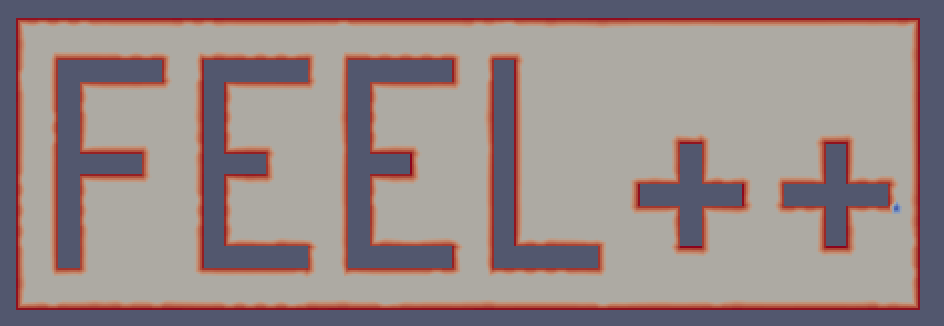
\includegraphics [width=200pt] {feel.png}
\end{center}
\end{figure}

\end{document}
